\begin{problem}{개미집}
	{standard input}{standard output}
	{3 seconds}{128 megabytes}{}
	
	개미들은 음식을 찾아 버려진 개미 언덕을 찾아 해매고 있다. 개미 언덕은 $n$개의 방과 방을 연결하는 $n-1$개의 통로로 이루어진다. 모든 방은 모든 다른 방으로의 통로로 이루어진 유일한 경로가 있다. 즉 방과 통로는 트리구조이다.
	
	개미 언덕의 통로 하나와만 연결된 모든 방에는 입구가 있다. 입구마다 각각 개미 $m_1$, $m_2$, $\cdots$, $m_g$ 마리로 이루어진 $g$개의 개미 그룹들이 있다. 이 그룹들은 각각 개미 언덕에 들어가고, 개미 언덕 안에 개미가 없어지면 다른 그룹이 들어가는 것을 반복한다. 개미 언덕 안에서, 개미는 다음과 같은 방법으로 탐험을 한다.:
	
	\begin{itemize}
		\item 개미 그룹이 한번도 탐험하지 않은 통로가 $d$개가 있는 방으로 들어가면, 개미 그룹은 각 통로에 $d$개의 크기가 같은 그룹으로 나뉘어진다. $d = 0$인 경우에는, 개미 그룹은 언덕을 나간다.
		\item 개미들이 같은 그룹으로 나누어 질 수 없는 크기라면, 힘이 센 개미가 약한 개미를 먹는다. 개미 그룹의 크기가 0이 될 수 있으니 항상 나누어 질 수 있다. 개미들이 같은 크기로 나누어지기 위해서는 자기 자신을 먹기도 한다.
	\end{itemize}
	
	다음 그림은 $m$마리의 개미가 세 개의 탐험하지 않은 통로가 있는 방으로 들어가, $\left\lfloor \dfrac{m}{3} \right\rfloor$마리로 나뉘는 그림이다. 
	 
	\begin{center}
		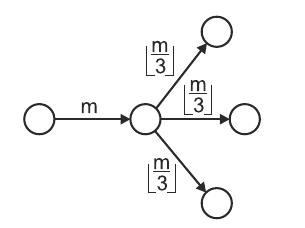
\includegraphics[]{mro1.png}
	\end{center}
	 
	
	배고픈 개미핥기는 통로중 하나를 파고 들어가서 개미들을 먹으려고 한다. 하지만 개미들 처럼 개미핥기도 숫자들에 대해 깐깐하기 때문에 그 통로를 지나는 개미가 정확히 $k$마리 일때만 개미들을 먹는다. 개미핥기가 몇 마리의 개미를 먹는지 구해주자. 
	
	
	\InputFile
	
	첫째 줄에는 세 개의 정수 $n$, $g$, $k$가 공백 하나로 구분되어 주어진다. ($2 \le n,g \le 1,000,000$, $1 \le k \le 10^9$) 이 숫자들은 각각 방의 수, 개미 그룹의 수, 개미핥기가 한번에 먹는 개미 수를 의미한다. 방은 1번부터 $n$번까지의 번호가 붙어있다.
	
	둘째 줄에는 $g$개의 수 $m_1$, $m_2$, $\cdots$, $m_g$($1 \le m_i \le 10^9$)가 공백 하나로 구분되어 주어진다. $m_i$는 $i$번째 그룹의 개미 수를 나타낸다. 다음 $n-1$개의 줄은 개미 언덕의 통로에 대한 정보가 주어진다. $n-1$개의 줄 중 $i$번째 줄은 두 정수 $a_i$와 $b_i$이 공백 하나로 구분되어 주어진다. ($1 \le a_i, b_i \le n$) 이것은 방 $a_i$와 방 $b_i$가 통로를 통해 이어져있다는 것을 의미한다. 개미핥기는 첫번째로 나타나는 통로를 파고 들어간다.
	
	\OutputFile
	첫째 줄에 개미핥기가 먹은 개미의 수를 나타내는 정수 하나를 출력하여라.  
	
	\SubtaskWithCost{1}{20}
	\begin{itemize}
		\item $n \le 100$
		\item $g \le 100$
	\end{itemize}
	
	\SubtaskWithCost{2}{50}
	\begin{itemize}
		\item 언덕에 들어가는 개미 그룹의 수는 1,000,000마리를 넘지 않는다.
	\end{itemize}
	
	\SubtaskWithCost{3}{30}
	
	추가 제한조건이 없다.
	
	\Examples
		
	\begin{example}
	\exmp{
7 5 3
3 4 1 9 11
1 2
1 4
4 3
4 5
4 6
6 7
	}{%
21
	}%
	\end{example}
	
	\Note
	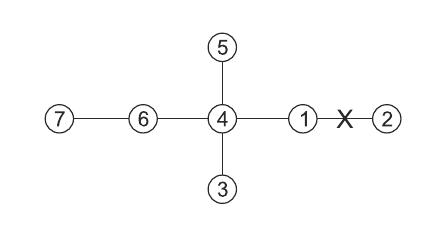
\includegraphics[]{mro2.png}
	
	각 입구는 방 2, 3, 5, 7 옆에 있고, 통로 옆에는 5 그룹의 개미들이 있다. 개미핥기는 2번 방에서 시작하는 첫번째 그룹의 개미들과, 3번, 5번, 7번 방에서 시작하는 4번째, 5번째 그룹의 개미들을 먹을 것이다. 
	
\end{problem}

